\documentclass{beamer}\usepackage{graphicx, color}
%% maxwidth is the original width if it is less than linewidth
%% otherwise use linewidth (to make sure the graphics do not exceed the margin)
\makeatletter
\def\maxwidth{ %
  \ifdim\Gin@nat@width>\linewidth
    \linewidth
  \else
    \Gin@nat@width
  \fi
}
\makeatother

\IfFileExists{upquote.sty}{\usepackage{upquote}}{}
\definecolor{fgcolor}{rgb}{0.2, 0.2, 0.2}
\newcommand{\hlnumber}[1]{\textcolor[rgb]{0,0,0}{#1}}%
\newcommand{\hlfunctioncall}[1]{\textcolor[rgb]{0.501960784313725,0,0.329411764705882}{\textbf{#1}}}%
\newcommand{\hlstring}[1]{\textcolor[rgb]{0.6,0.6,1}{#1}}%
\newcommand{\hlkeyword}[1]{\textcolor[rgb]{0,0,0}{\textbf{#1}}}%
\newcommand{\hlargument}[1]{\textcolor[rgb]{0.690196078431373,0.250980392156863,0.0196078431372549}{#1}}%
\newcommand{\hlcomment}[1]{\textcolor[rgb]{0.180392156862745,0.6,0.341176470588235}{#1}}%
\newcommand{\hlroxygencomment}[1]{\textcolor[rgb]{0.43921568627451,0.47843137254902,0.701960784313725}{#1}}%
\newcommand{\hlformalargs}[1]{\textcolor[rgb]{0.690196078431373,0.250980392156863,0.0196078431372549}{#1}}%
\newcommand{\hleqformalargs}[1]{\textcolor[rgb]{0.690196078431373,0.250980392156863,0.0196078431372549}{#1}}%
\newcommand{\hlassignement}[1]{\textcolor[rgb]{0,0,0}{\textbf{#1}}}%
\newcommand{\hlpackage}[1]{\textcolor[rgb]{0.588235294117647,0.709803921568627,0.145098039215686}{#1}}%
\newcommand{\hlslot}[1]{\textit{#1}}%
\newcommand{\hlsymbol}[1]{\textcolor[rgb]{0,0,0}{#1}}%
\newcommand{\hlprompt}[1]{\textcolor[rgb]{0.2,0.2,0.2}{#1}}%

\usepackage{framed}
\makeatletter
\newenvironment{kframe}{%
 \def\at@end@of@kframe{}%
 \ifinner\ifhmode%
  \def\at@end@of@kframe{\end{minipage}}%
  \begin{minipage}{\columnwidth}%
 \fi\fi%
 \def\FrameCommand##1{\hskip\@totalleftmargin \hskip-\fboxsep
 \colorbox{shadecolor}{##1}\hskip-\fboxsep
     % There is no \\@totalrightmargin, so:
     \hskip-\linewidth \hskip-\@totalleftmargin \hskip\columnwidth}%
 \MakeFramed {\advance\hsize-\width
   \@totalleftmargin\z@ \linewidth\hsize
   \@setminipage}}%
 {\par\unskip\endMakeFramed%
 \at@end@of@kframe}
\makeatother

\definecolor{shadecolor}{rgb}{.97, .97, .97}
\definecolor{messagecolor}{rgb}{0, 0, 0}
\definecolor{warningcolor}{rgb}{1, 0, 1}
\definecolor{errorcolor}{rgb}{1, 0, 0}
\newenvironment{knitrout}{}{} % an empty environment to be redefined in TeX

\usepackage{alltt}
\usetheme{Stats}
\setbeamercovered{transparent}
\usepackage{color}
\usepackage{hyperref}
  \hypersetup{
  	colorlinks=true
		linkcolor=black
		}
\usepackage{url}
\usepackage{graphics}
\usepackage{tikz}
\usepackage{booktabs}
\usepackage{multirow}
\usepackage[buttonsize=1em]{animate}





%%%%%%%%%%%%%%%%%%%%%%%%%%%%%%%% Title Slide %%%%%%%%%%%%%%%%%%%%%%%%%%
\title[]{Intro to Social Science Data Analysis \\[1cm] Lecture 9: Statistical Inference with Large Samples}
\author[]{
    \href{mailto:gandrud@yonsei.ac.kr}{Christopher Gandrud}
}
\date{\today}


\begin{document}

\frame{\titlepage}

\section[Outline]{}
\frame{\tableofcontents}

%%%%%%%%%%% Assignment 3
\section{Assignment 3}
\frame{
	\frametitle{Assignment 3}

}

%%%%%%%%%%% Recap
\section{Recap}
\frame{
  \frametitle{Intro to Statistical Inference: Quick Quiz (1)}
  Give an example of a population parameter and its corresponding point estimate.
}

\frame{
  \frametitle{Intro to Statistical Inference: Quick Quiz (2)}
  What is the sampling distribution of the sampling mean? \\[0.5cm]
  In general, what is the sampling distribution of the sampling mean centered on?
}

\frame{
  \frametitle{Intro to Statistical Inference: Quick Quiz (3)}
  What do we use to find the standard error of a point estimate? \\[0.5cm]
  What do we use the standard error for?
}

\frame{
  \frametitle{Intro to Statistical Inference: Quick Quiz (4)}
  What is a confidence interval? \\[0.5cm]
  Why is it more useful to show the confidence interval than just the standard error?
}

\frame{
  \frametitle{Today}
{\Large{Last class we largely looked at how to draw inferences about a population {\bf{mean}} from a sample {\bf{mean}}. \\[0.5cm]
  Today we will expand our inferential tools by learning about:
  \begin{itemize}
    \item Hypothesis testing \& p-values,
    \item Comparing 2 population means,
    \item Making inferences with population proportions,
    \item Inferential statistics with categorical variables.
  \end{itemize}
  }}
}

%%%%%%%%%%% Hypothesis testing
\section{Hypothesis Testing}
\begin{frame}[fragile]
  \frametitle{Hypothesis Testing Setup}
  {\large{Imagine that we have a sample of 200 Cherrry Blossom Run Finishing times from the 2009 race. \\[0.25cm] (This example is largely from Diaz et al. 2011. See last week's lecture for more details) \\[0.5cm]



  The mean finishing time in the sample is 95.5 minutes with a standard deviation of 16.1}}
\end{frame}

\frame{
  \frametitle{Question}
{\Large{The mean finishing time in 2006 was 93.29. \\[0.5cm]
  Is there strong evidence that on average the 2009 runners are faster/slower than the 2006 runners?}}
}

\frame{
  \frametitle{The language of hypothesis testing.}
  {\large{We can think that there are two {\bf{competing}} possibilities: \\[0.5cm]
  \begin{itemize}
    \item $H_{0}$: There is {\emph{no difference}} in the average finishing times between the 2006 and 2009 runners ({\bf{the null hypothesis}}).
    \item $H_{a}$: The average finishing time in 2006 {\emph{is different}} from the average finishing time in 2009 ({\bf{the alternative hypothesis}}). 
  \end{itemize}
  }}
}

\frame{
  \frametitle{The language of hypothesis testing}
{\large{In other words, if the population mean for the 2009 is called $\mu_{09}$: \\[0.5cm]
  \begin{itemize}
    \item $H_{0}: \mu_{09} = 93.29$
    \item $H_{A}: \mu_{09} \neq 93.29$
  \end{itemize} \\[0.5cm]
  93.29 is called the {\bf{null value}}, as it is the value of the parameter {\bf{if}} the null hypothesis is true.
}}
}

\frame{
  \frametitle{The language of hypothesis testing}
{\large{The null hypothesis is the {\bf{skeptical possibility}}. \\[0.5cm]
  If we do not find evidence against the null hypothesis we say that we: {\emph{fail to reject the null hypothesis.}} \\[0.5cm]
  If we do find evidence against the null hypothesis we say that we: {\emph{found evidence for the alternative hypothesis.}}
  }}
}

\frame{
  \frametitle{Evidence}
{\Large{What kind of evidence can we use to either reject or fail to reject the null hypothesis?}}
}

\frame{
  \frametitle{Evidence}
  \begin{center}
{\Large{Confidence intervals!}}
  \end{center}
}

\begin{frame}[fragile]
  \frametitle{95\% Confidence Inverval for 2009 Mean Finishing Times ($n = 200$)}
\begin{knitrout}
\definecolor{shadecolor}{rgb}{0.969, 0.969, 0.969}\color{fgcolor}

{\centering 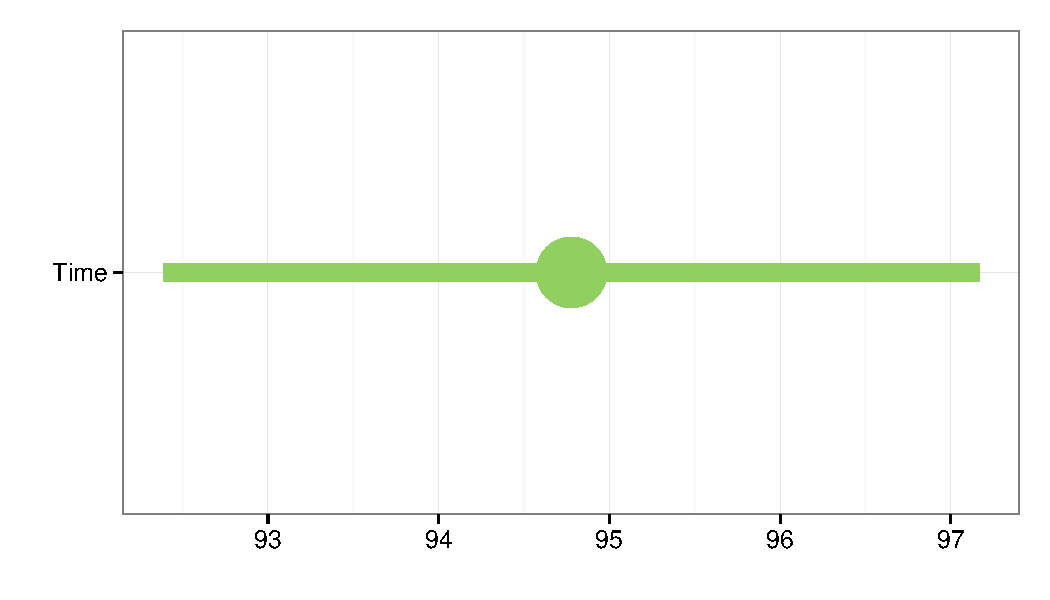
\includegraphics[width=\maxwidth]{figure/TimeCI} 

}


\end{knitrout}

\end{frame}

\begin{frame}[fragile]
  \frametitle{95\% Confidence Inverval for 2009 Mean Finishing Times ($n = 200$) Compared to the Null Hypothesis}
\begin{knitrout}
\definecolor{shadecolor}{rgb}{0.969, 0.969, 0.969}\color{fgcolor}

{\centering 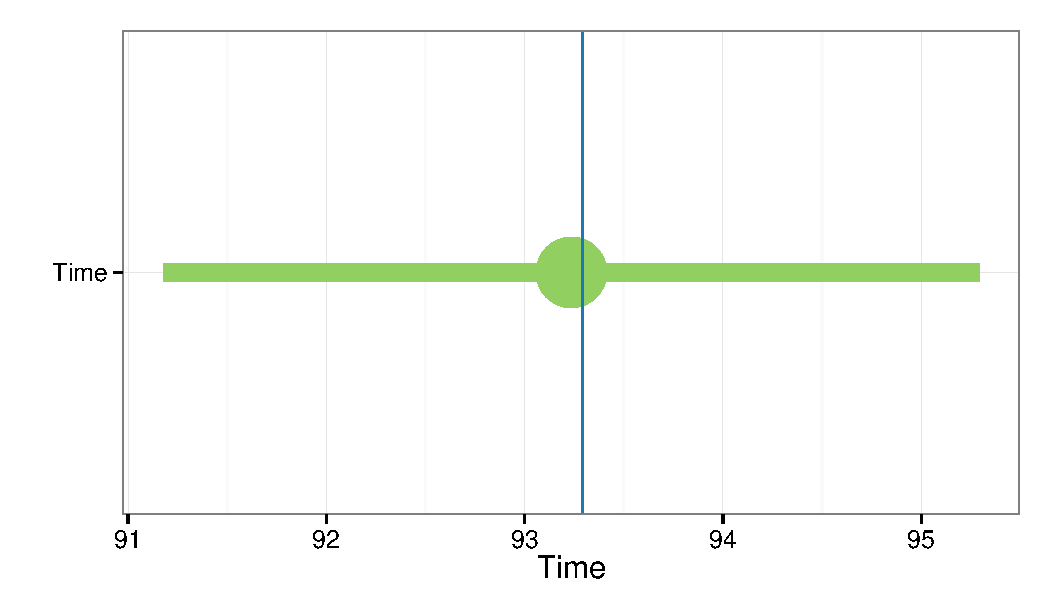
\includegraphics[width=\maxwidth]{figure/TimeCINull} 

}


\end{knitrout}

\end{frame}

\frame{
  \frametitle{Fail to Reject}
{\Large{The 2006 population mean is inside of the 95\% confidence interval of the 2009 sample estimate. \\[0.5cm]
  Therefore, we {\emph{fail to reject}} the null hypothesis that the 2009 Cherry Blossom Run mean finishing time is different from the 2006 mean finishing time.}}
}

\frame{
  \frametitle{Be Careful}
{\Large{Be Careful: Hypothesis testing is far from perfect. \\[0.5cm]  
  }}
{\small{
  \begin{table}
    \begin{tabular}{c c | c c}
    & & \multicolumn{2}{c}{{\bf{Test Conclusion}}} \\[0.25cm]
    \hline
    & & Do Not Reject $H_{0}$ & Reject Infavour of $H_{A}$ \\[0.25cm]
    \hline
    \multirow{2}{*}{{\bf{Real World}}} & $H_{0}$ True & okay & Type 1 Error \\[0.25cm]
    & $H_{A}$ True & Type II Error & okay \\
    \hline
    \end{tabular}

  \end{table}
  (Diaz et al. 2001, 160)
}}
}

\frame{
  \frametitle{Quantifying Error Probabilities}
  We previously used a 95\% confidence interval to test the Null Hypothesis. \\[0.5cm]
  This means that 5\% of the time we will {\bf{incorrectly}} reject $H_{0}$ due to {\bf{sampling variation}}. \\[0.25cm]
  2.5\% of the time the confidence interval will be {\bf{too high}}. \\
  2.5\% of the time the confidence interval will be {\bf{too low}}.\\[0.5cm]
  This is called the 95\% {\bf{significance level}} or sometimes $\alpha = 0.05$.
}

\begin{frame}[fragile]
  \frametitle{Remember: Confidence Interval Simulation}
\begin{knitrout}
\definecolor{shadecolor}{rgb}{0.969, 0.969, 0.969}\color{fgcolor}

{\centering \animategraphics[,controls,loop]{1}{figure/CIRememberAnimation}{1}{50}

}


\end{knitrout}

\end{frame}

\frame{
  \frametitle{Higher Confidence}
  {\Large{If we use a {\bf{higher significance level}} we will be more confident that we correctly rejected or failed to reject the null hypothesis. \\[0.5cm]
  For example, at the 99\% significance level we will incorrectly reject the $H_{0}$ 1\% of the time.}}
}

%%%%%%%%%%%% p-values
\section{p-values}
\frame{
  \frametitle{p-values}
  {\Large{Some researchers like to quantify the strength of the evidence against the Null Hypothesis with a tool called the {\bf{p-value}}.}}
}

\frame{
  \frametitle{What is the p-value}
{\LARGE{p-value}} \\[0.5cm]
  The probability of seeing data at least as favourable to the alternative hypothesis as our current data, {\emph{if the null hypothesis is true}}.
}

\frame{
  \frametitle{Question}
  \begin{center}
{\Large{Using p-values to comparing means: \\[0.5cm]
  Are men's finishing times different than women's finishing time in the 2009 Cherry Blossom Run?}}
  \end{center}
}

\frame{
  \frametitle{}
  \begin{center}
{\Large{First the Descriptive Statistics}}
  \end{center}
}

\begin{frame}[fragile,plain]
\begin{knitrout}
\definecolor{shadecolor}{rgb}{0.969, 0.969, 0.969}\color{fgcolor}\begin{kframe}
\begin{alltt}
\hlcomment{#### Summary of Men's Times #### Subset sample to}
\hlcomment{#### include only men's Times}
MenSubset <- \hlfunctioncall{subset}(Run10Samp$time, Run10Samp$gender == 
    \hlstring{"M"})
\hlcomment{# Mean}
Mean <- \hlfunctioncall{mean}(MenSubset)
\hlcomment{# Standard Deviation}
SD <- \hlfunctioncall{sd}(MenSubset)
\hlcomment{# Number of observations}
N <- \hlfunctioncall{length}(MenSubset)
\hlcomment{# Create Gender Variable}
Gender <- \hlstring{"Male"}
\hlcomment{# Combine}
GenderData <- \hlfunctioncall{data.frame}(Gender, Mean, SD, N)
\end{alltt}
\end{kframe}
\end{knitrout}

\end{frame}

\begin{frame}[fragile,plain]
\begin{knitrout}
\definecolor{shadecolor}{rgb}{0.969, 0.969, 0.969}\color{fgcolor}\begin{kframe}
\begin{alltt}
\hlcomment{#### Summary of Women's Times #### Subset sample}
\hlcomment{#### to include only women's Times}
WomenSubset <- \hlfunctioncall{subset}(Run10Samp$time, Run10Samp$gender == 
    \hlstring{"F"})
\hlcomment{# Mean}
Mean <- \hlfunctioncall{mean}(WomenSubset)
\hlcomment{# Standard Deviation}
SD <- \hlfunctioncall{sd}(WomenSubset)
\hlcomment{# Number of observations}
N <- \hlfunctioncall{length}(WomenSubset)
\hlcomment{# Create Gender Variable}
Gender <- \hlstring{"Female"}
\hlcomment{# Combine}
GenderDataF <- \hlfunctioncall{data.frame}(Gender, Mean, SD, N)

\hlcomment{# Combine into one data frame}
GenderData <- \hlfunctioncall{data.frame}(\hlfunctioncall{rbind}(GenderData, GenderDataF))
\end{alltt}
\end{kframe}
\end{knitrout}

\end{frame}

\begin{frame}[fragile]
  \frametitle{Summary Descriptives}
  \begin{table}
  \caption{Descriptive Statistics of the Sample}
  \begin{tabular}{c | c c c}
  & $\bar{x}$ & $s$ & $n$ \\
  \hline\hline
  Female & 100.7 & 15.3 & 101 \\
  Male & 90.2 & 15.1 & 99 \\
  \hline
  
  \end{tabular}
  \end{table}
\end{frame}

\begin{frame}[fragile,plain]
\begin{knitrout}
\definecolor{shadecolor}{rgb}{0.969, 0.969, 0.969}\color{fgcolor}\begin{kframe}
\begin{alltt}
\hlcomment{# Compare densities of Men/Women Times}
\hlfunctioncall{ggplot}(Run10Samp, \hlfunctioncall{aes}(time)) +
        \hlfunctioncall{geom_density}(\hlfunctioncall{aes}(
          line = gender, color = gender)) +
        \hlfunctioncall{theme_bw}()
\end{alltt}
\end{kframe}

{\centering 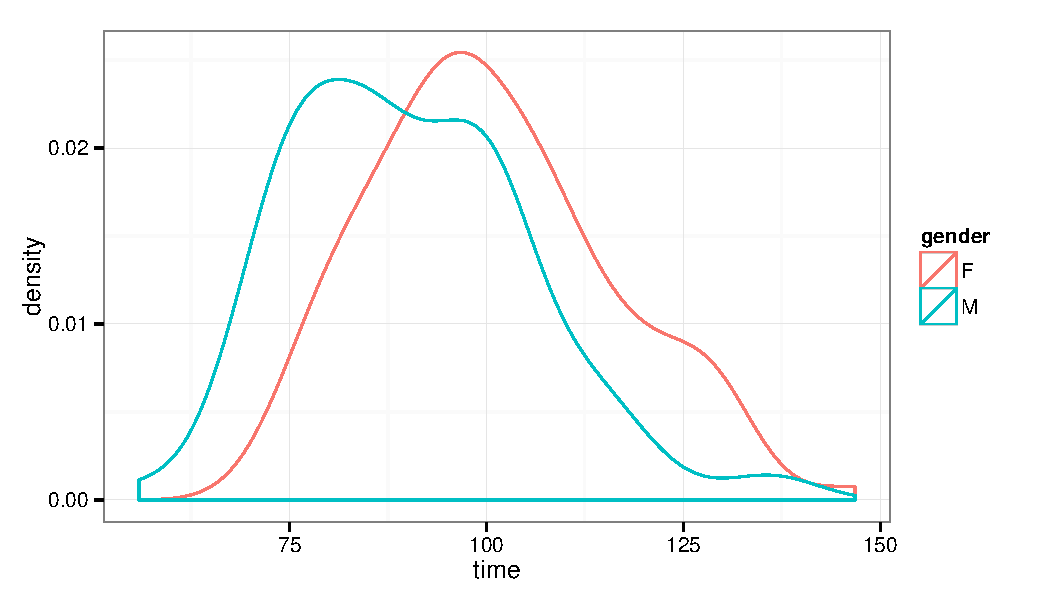
\includegraphics[width=\maxwidth]{figure/GenderDist} 

}


\end{knitrout}

\end{frame}

\frame{
  \frametitle{Comparing Means: Hypothesis Testing}
  {\Large{Null Hypothesis: $\mu_{men} = \mu_{women}$ \\[0.25cm]
  Alternative Hypothesis: $\mu_{men} \neq \mu_{women}$ \\[0.5cm]
  An equivalent way to write this null hypothesis is: $\mu_{men} - \mu_{women} = 0$
  }}
}


\begin{frame}[allowframebreaks]
  \frametitle{References}
  Diaz, David M., Christopher D. Barr, and Mine \c{C}etinkaya-Rundel. 2011. OpenIntro Statistics. 1st ed. \url{http://www.openintro.org/stat/downloads.php}. \\[0.25cm] 
\end{frame}


\end{document}
